% 若编译失败,且生成 .synctex(busy) 辅助文件,可能有两个原因:
% 1. 需要插入的图片不存在:Ctrl + F 搜索 'figure' 将这些代码注释/删除掉即可
% 2. 路径/文件名含中文或空格:更改路径/文件名即可


% --------------------- 文章宏包及相关设置 --------------------- %
% >> ------------------ 文章宏包及相关设置 ------------------ << %
% 设定文章类型与编码格式
    \documentclass[UTF8]{report}		

% 本文特殊宏包
    \usepackage{siunitx} % 埃米单位

% 自定义宏定义
    \def\N{\mathbb{N}}
    \def\F{\mathbb{F}}
    \def\Z{\mathbb{Z}}
    \def\Q{\mathbb{Q}}
    \def\R{\mathbb{R}}
    \def\C{\mathbb{C}}
    \def\T{\mathbb{T}}
    \def\S{\mathbb{S}}
    \def\A{\mathbb{A}}
    \def\I{\mathscr{I}}
    \def\d{\mathrm{d}}
    \def\p{\partial}


% 导入基本宏包
    \usepackage[UTF8]{ctex}     % 设置文档为中文语言
    \usepackage[colorlinks, linkcolor=blue, anchorcolor=blue, citecolor=blue, urlcolor=blue]{hyperref}  % 宏包:自动生成超链接 (此宏包与标题中的数学环境冲突)
    % \usepackage{docmute}    % 宏包:子文件导入时自动去除导言区,用于主/子文件的写作方式,\include{./51单片机笔记}即可。注:启用此宏包会导致.tex文件capacity受限。
    \usepackage{amsmath}    % 宏包:数学公式
    \usepackage{mathrsfs}   % 宏包:提供更多数学符号
    \usepackage{amssymb}    % 宏包:提供更多数学符号
    \usepackage{pifont}     % 宏包:提供了特殊符号和字体
    \usepackage{extarrows}  % 宏包:更多箭头符号
    \usepackage{multicol}   % 宏包:支持多栏 


% 文章页面margin设置
    \usepackage[a4paper]{geometry}
        \geometry{top=1in}
        \geometry{bottom=1in}
        \geometry{left=0.75in}
        \geometry{right=0.75in}   % 设置上下左右页边距
        \geometry{marginparwidth=1.75cm}    % 设置边注距离(注释、标记等)

% 配置数学环境
    \usepackage{amsthm} % 宏包:数学环境配置
    % theorem-line 环境自定义
        \newtheoremstyle{MyLineTheoremStyle}% <name>
            {11pt}% <space above>
            {11pt}% <space below>
            {}% <body font> 使用默认正文字体
            {}% <indent amount>
            {\bfseries}% <theorem head font> 设置标题项为加粗
            {:}% <punctuation after theorem head>
            {.5em}% <space after theorem head>
            {\textbf{#1}\thmnumber{#2}\ \ (\,\textbf{#3}\,)}% 设置标题内容顺序
        \theoremstyle{MyLineTheoremStyle} % 应用自定义的定理样式
        \newtheorem{LineTheorem}{Theorem.\,}
    % theorem-block 环境自定义
        \newtheoremstyle{MyBlockTheoremStyle}% <name>
            {11pt}% <space above>
            {11pt}% <space below>
            {}% <body font> 使用默认正文字体
            {}% <indent amount>
            {\bfseries}% <theorem head font> 设置标题项为加粗
            {:\\ \indent}% <punctuation after theorem head>
            {.5em}% <space after theorem head>
            {\textbf{#1}\thmnumber{#2}\ \ (\,\textbf{#3}\,)}% 设置标题内容顺序
        \theoremstyle{MyBlockTheoremStyle} % 应用自定义的定理样式
        \newtheorem{BlockTheorem}[LineTheorem]{Theorem.\,} % 使用 LineTheorem 的计数器
    % definition 环境自定义
        \newtheoremstyle{MySubsubsectionStyle}% <name>
            {11pt}% <space above>
            {11pt}% <space below>
            {}% <body font> 使用默认正文字体
            {}% <indent amount>
            {\bfseries}% <theorem head font> 设置标题项为加粗
            {:\\ \indent}% <punctuation after theorem head>
            {0pt}% <space after theorem head>
            {\textbf{#3}}% 设置标题内容顺序
        \theoremstyle{MySubsubsectionStyle} % 应用自定义的定理样式
        \newtheorem{definition}{}

%宏包:有色文本框(proof环境)及其设置
    \usepackage[dvipsnames,svgnames]{xcolor}    %设置插入的文本框颜色
    \usepackage[strict]{changepage}     % 提供一个 adjustwidth 环境
    \usepackage{framed}     % 实现方框效果
        \definecolor{graybox_color}{rgb}{0.95,0.95,0.96} % 文本框颜色。修改此行中的 rgb 数值即可改变方框纹颜色,具体颜色的rgb数值可以在网站https://colordrop.io/ 中获得。(截止目前的尝试还没有成功过,感觉单位不一样)(找到喜欢的颜色,点击下方的小眼睛,找到rgb值,复制修改即可)
        \newenvironment{graybox}{%
        \def\FrameCommand{%
        \hspace{1pt}%
        {\color{gray}\small \vrule width 2pt}%
        {\color{graybox_color}\vrule width 4pt}%
        \colorbox{graybox_color}%
        }%
        \MakeFramed{\advance\hsize-\width\FrameRestore}%
        \noindent\hspace{-4.55pt}% disable indenting first paragraph
        \begin{adjustwidth}{}{7pt}%
        \vspace{2pt}\vspace{2pt}%
        }
        {%
        \vspace{2pt}\end{adjustwidth}\endMakeFramed%
        }

% 外源代码插入设置
    % matlab 代码插入设置
    \usepackage{matlab-prettifier}
        \lstset{
            style=Matlab-editor,  % 继承matlab代码颜色等
        }
    \usepackage[most]{tcolorbox} % 引入tcolorbox包 
    \usepackage{listings} % 引入listings包
        \tcbuselibrary{listings, skins, breakable}
        \lstdefinestyle{matlabstyle}{
            language=Matlab,
            basicstyle=\small,
            breakatwhitespace=false,
            breaklines=true,
            captionpos=b,
            keepspaces=true,
            numbers=left,
            numbersep=15pt,
            showspaces=false,
            showstringspaces=false,
            showtabs=false,
            tabsize=2
        }
        \newtcblisting{matlablisting}{
            arc=0pt,
            top=0pt,
            bottom=0pt,
            left=1mm,
            listing only,
            listing style=matlabstyle,
            breakable,
            colback=white   % 选一个合适的颜色
        }

% table 支持
    \usepackage{booktabs}   % 宏包:三线表
    \usepackage{tabularray} % 宏包:表格排版
    \usepackage{longtable}  % 宏包:长表格

% figure 设置
    \usepackage{graphicx}  % 支持 jpg, png, eps, pdf 图片 
    \usepackage{svg}       % 支持 svg 图片
        \svgsetup{
            % 指向 inkscape.exe 的路径
            inkscapeexe = D:/aa_my_apps_main/Inkscape/bin/inkscape.exe, 
            % 一定程度上修复导入后图片文字溢出几何图形的问题
            inkscapelatex = false                 
        }

% 图表进阶设置
    \usepackage{caption}    % 图注、表注
        \captionsetup[figure]{name=图}  
        \captionsetup[table]{name=表}
        \captionsetup{labelfont=bf, font=small}
    \usepackage{float}     % 图表位置浮动设置 

% 圆圈序号自定义
    \newcommand*\circled[1]{\tikz[baseline=(char.base)]{\node[shape=circle,draw,inner sep=0.8pt, line width = 0.03em] (char) {\small \bfseries #1};}}   % TikZ solution

% 列表设置
    \usepackage{enumitem}   % 宏包:列表环境设置
        \setlist[enumerate]{itemsep=0pt, parsep=0pt, topsep=0pt, partopsep=0pt, leftmargin=3.5em} 
        \setlist[itemize]{itemsep=0pt, parsep=0pt, topsep=0pt, partopsep=0pt, leftmargin=3.5em}
        \newlist{circledenum}{enumerate}{1} % 创建一个新的枚举环境  
        \setlist[circledenum,1]{  
            label=\protect\circled{\arabic*}, % 使用 \arabic* 来获取当前枚举计数器的值,并用 \circled 包装它  
            ref=\arabic*, % 如果需要引用列表项,这将决定引用格式(这里仍然使用数字)
            itemsep=0pt, parsep=0pt, topsep=0pt, partopsep=0pt, leftmargin=3.5em
        }  

% 其它设置
    % 脚注设置
    \renewcommand\thefootnote{\ding{\numexpr171+\value{footnote}}}
    % 参考文献引用设置
        \bibliographystyle{unsrt}   % 设置参考文献引用格式为unsrt
        \newcommand{\upcite}[1]{\textsuperscript{\cite{#1}}}     % 自定义上角标式引用
    % 文章序言设置
        \newcommand{\cnabstractname}{序言}
        \newenvironment{cnabstract}{%
            \par\Large
            \noindent\mbox{}\hfill{\bfseries \cnabstractname}\hfill\mbox{}\par
            \vskip 2.5ex
            }{\par\vskip 2.5ex}

% 文章默认字体设置
\usepackage{fontspec}   % 宏包:字体设置
    \setmainfont{SimSun}    % 设置中文字体为宋体字体
    \setmainfont{Times New Roman} % 设置英文字体为Times New Roman

% 各级标题自定义设置
\usepackage{titlesec}   
\titleformat{\chapter}[hang]{\normalfont\huge\bfseries\centering}{第\,\thechapter\,章}{20pt}{}
\titlespacing*{\chapter}{0pt}{-20pt}{20pt} % 控制上方空白的大小
% section标题自定义设置 
\titleformat{\section}[hang]{\normalfont\Large\bfseries}{§\,\thesection\,}{8pt}{}
% subsubsection标题自定义设置
%\titleformat{\subsubsection}[hang]{\normalfont\bfseries}{}{8pt}{}

% --------------------- 文章宏包及相关设置 --------------------- %
% >> ------------------ 文章宏包及相关设置 ------------------ << %

% ------------------------ 文章信息区 ------------------------ %
% ------------------------ 文章信息区 ------------------------ %
% 页眉页脚设置
    \usepackage{fancyhdr}   %宏包:页眉页脚设置
        \pagestyle{fancy}
        \fancyhf{}
        \cfoot{\thepage}
        \renewcommand\headrulewidth{1pt}
        \renewcommand\footrulewidth{0pt}
        \lhead{2024.8-2025.1} 
        \chead{光学笔记(Optics Notes)}    
        \rhead{dingyi233@mails.ucas.ac.cn}
%文档信息设置
    \title{光学笔记\\Optics Notes}
    \author{丁毅\\ \footnotesize 中国科学院大学,北京 100049\\ Yi Ding \\ \footnotesize University of Chinese Academy of Sciences, Beijing 100049, China}
    \date{\footnotesize 2024.8 -- 2025.1}
% ------------------------ 文章信息区 ------------------------ %
% ------------------------ 文章信息区 ------------------------ %

% 开始编辑文章

\begin{document} 
\zihao{5}           % 设置全文字号大小

% ------------------------ 封面序言与目录 ------------------------ %
% >> --------------------- 封面序言与目录 --------------------- << %
% 封面
    \maketitle\newpage  
    \pagenumbering{Roman} % 页码为大写罗马数字
    \thispagestyle{fancy}   % 显示页码、页眉等

% 序言
    \begin{cnabstract}\normalsize 
        本文为笔者本科时的“光学”课程笔记(Notes of Optics, 2024.8-2025.1)。由于个人学识浅陋,认识有限,文中难免有不妥甚至错误之处,望读者不吝指正,在此感谢。\par
        我的邮箱是 dingyi233@mails.ucas.ac.cn。
    \end{cnabstract}
    \addcontentsline{toc}{chapter}{序言} % 手动添加为目录

% 目录
    \setcounter{tocdepth}{2}                % 目录深度(为1时显示到section)
    \tableofcontents                        % 目录页
    \addcontentsline{toc}{chapter}{目录}    % 手动添加此页为目录
    \thispagestyle{fancy}                   % 显示页码、页眉等 

% 收尾工作
    \newpage    
    \pagenumbering{arabic} 


% >> --------------------- 封面序言与目录 --------------------- << %
% ------------------------ 封面序言与目录 ------------------------ %

为了更好的学习光学,建议先跳转至附录

\chapter{光学导言}

\section{光学发展简史(略)}
\section{费马原理}

\subsection{光的几何传播规律}

\begin{definition}[光传播的基本原理]
光传播的常见基本原理:
\begin{enumerate}
    \item 直线传播:光在均匀介质里沿直线传播 \footnote{对高功率激光,此定律不成立}
    \item 反射定律:光线入射到两种不同的均匀介质的分界面上反射线位于入射面内,反射线和入射线分居法线两侧,反射角等于入射角
    \item 折射定律(斯涅尔定律):折射线位于入射面内,折射线与入射线分居法线两侧,入射角的正弦与折射角的正弦
    之比为一与入射角无关的常数 \footnote{折射率较大的一侧称为光密介质;较小的一侧称为光疏介质}
    \begin{equation}
    n_1\sin i_1 = n_2 \sin i_2
    \end{equation}
    
    \begin{figure}[H]\centering
    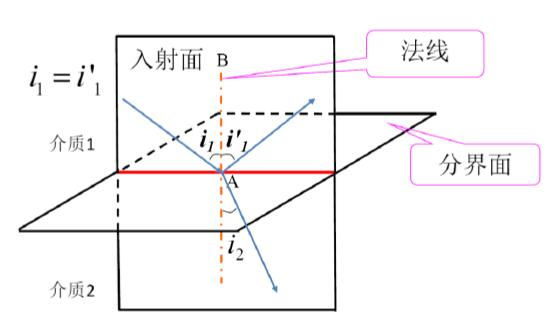
\includegraphics[width=0.4\textwidth]{assets/image (44).jpg}
    \caption{\textbf{反射与折射}}\label{反射与折射}
    \end{figure}
    
    \item 光路可逆性:光沿反方向传播时,必定沿原光路返回 \footnote{也即在几何光学中,任何光路都是可逆的}
    \item 独立传播:光在传播过程中与其他光束相遇时,各光束都各自独立传播,不改变其传播方向
    \item 全反射:光线从光密介质入射到光疏介质,当入射角大于某临界值时,折射光完
    全消失,只剩下反射光。该临界角度称为全反射临界角。
    \begin{equation}
    i_C = \arcsin (\frac{n_1}{n_2})\quad n_1<n_2
    \end{equation}
\end{enumerate}
\end{definition}


\begin{definition}[彩虹]
\end{definition}


\begin{definition}[三棱镜最小偏向角]

最小偏向角 $\theta_0 = (i_1 - i_1')_{\text{min}}$ 满足:
\begin{equation}
    \theta_0 = 2i_1 - A, \quad \frac{n_2}{n_1} = \frac{\sin\frac{\theta_0+A}2}{\sin\frac A2}
\end{equation}

\begin{figure}[H]\centering
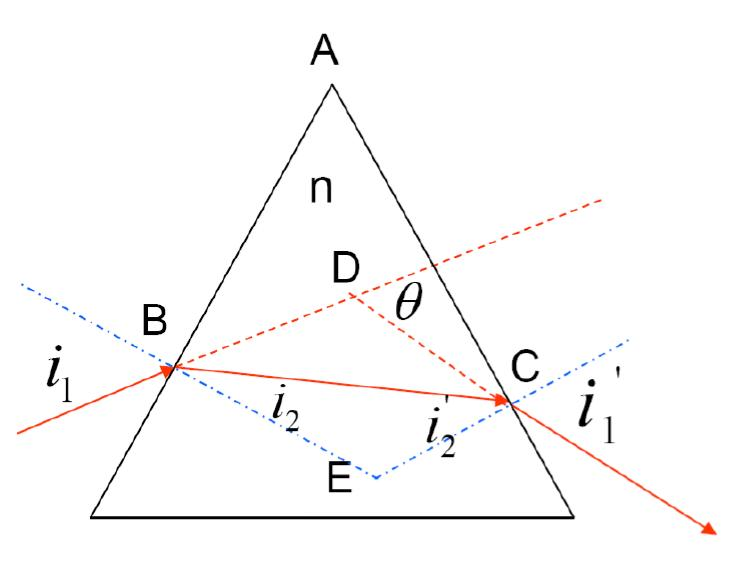
\includegraphics[width=0.4\textwidth]{assets/image (45).jpg}
\caption{\textbf{三棱镜最小偏向角}}\label{三棱镜最小偏向角}
\end{figure}

\end{definition}

\subsection{惠更斯原理}

\begin{LineTheorem}[惠更斯原理]\label{LineTheorem: 惠更斯原理}
    由振源发出的波动在 $t$ 时刻传播到一个波面 $S$,波面上的每一个面元可认为是次波的波源。由面元发出的次波向四面八方传播。在以后的时刻 $t'$ 形成次波面。这些次波面的包络面 $S'$ 就是 $t'$ 时刻总扰动的波面。
\end{LineTheorem}

\noindent 其中:
\begin{enumerate}
    \item 波面:在同一振源的波场中,扰动同时到达的各点具有相同的相位,这些点的轨迹构成一个曲面(平面波是曲线),称为波面(也称为波阵面、波前)\footnote{对平面波而言,波面虽然称为“面”,但实际上是一条条曲线}
    \item 波线:取波面被某个平面所截得到的等高线,与此等高线处处正交的曲线称为波线,其切线方向为光的传播方向
\end{enumerate}

\noindent 几何光学的定律需要前提条件:
\begin{enumerate}
\item 必须是均匀介质,即同一介质的折射率处处相等,折射率不是位置的函数。
\item 必须是各向同性介质,即光在介质中传播时各个方向的折射率相等,折射率不是方向的函数。
\item 光强不能太强,否则巨大的光能量会使线性叠加原理不再成立而出现非线性情况。
\item 光学元件的线度应比光的波长大得多,否则不能把光束简化为光线。
\end{enumerate}

\begin{figure}[H]\centering
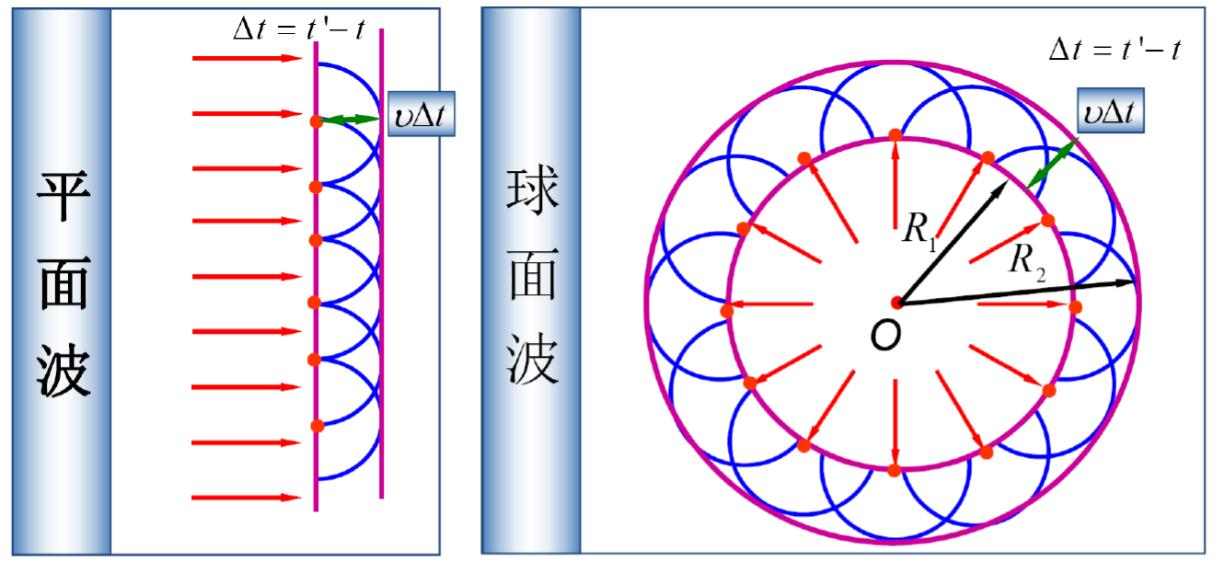
\includegraphics[width=0.5\textwidth]{assets/image (46).jpg}
\caption{\textbf{惠更斯原理}}\label{惠更斯原理}
\end{figure}

\subsection{费马原理}

\begin{BlockTheorem}[费马原理]\label{费马原理}
光从空间中一点传播到另一点时,总是沿光程(optical length, OPL)取极值的路径传播 \footnote{这里的“极值”可以是极小值、极大值或常数,一般情况下,实际光程大多取极小值。极大值(如凹面镜成像)、拐点(如椭球面镜、凸透镜)的例子,可以参考 \href{https://zhuanlan.zhihu.com/p/107739173}{知乎:浅谈几何光学(1)——费马原理}},公式:
\begin{equation}
    \mathrm{d}\left(\int\limits_{Q}^{P}ndl\right)=0
\end{equation}
\end{BlockTheorem}
由费马原理可以导出诸多推论,包括我们熟知的几条基本原理,还有物像之间的等光程性(例如凸透镜):
在物点Q与像点Q’之间,不管光线经何路径,凡是由Q通过同样的光学系统到达Q’的光线,都是等光程的。

\subsection{成像}
\subsection{薄透镜}
\subsection{光学仪器}
\subsection{光波的描述}
\subsection{光度学基本概念}

\chapter{}
\chapter{}
\chapter{}
\chapter{} 
\chapter{}







































































































































\nocite{*}
\bibliography{re}
\thispagestyle{fancy} 
\addcontentsline{toc}{chapter}{参考文献}




\newpage
\appendix
% chapter 标题自定义设置
\titleformat{\chapter}[hang]{\normalfont\huge\bfseries\centering}{}{20pt}{}
\titlespacing*{\chapter}{0pt}{-25pt}{8pt} % 控制上方空白的大小
% section 标题自定义设置 
\titleformat{\section}[hang]{\normalfont\centering\Large\bfseries}{\thesection}{8pt}{}

% 附录 A
\chapter*{附录 A. 波理论}\addcontentsline{toc}{chapter}{附录 A. 波理论}   
\thispagestyle{fancy} 
\setcounter{section}{0}   
\renewcommand\thesection{A.\arabic{section}}   
\renewcommand{\thefigure}{A.\arabic{figure}} 
\renewcommand{\thetable}{A.\arabic{table}}


光的真实本性是光学的全部讨论的中心问题, 在本书中我们从头到尾都得对待这个问题。“光究竟是一种波动现象还是一种粒子现象?” 这个似乎干脆利索的问题, 远比它初看之下复杂得多。

因为对光的经典讨论和量子力学讨论都要用到波的数学描述, 本章要为这两种表述所需
要的东西打好基础。下面叙说的想法将用于一切物理波, 从一杯茶的表面张力皱波, 到从某个遥远的星系照到我们的光脉冲。

\section{一维波}


\begin{definition}[一维波的形式]
一维波函数的最一般的形式:
\begin{equation}
\psi(x,t) = f(x-vt) = g(t - \frac{x}{v})
\end{equation}

具体而言,对于给定的波形(波的形状),我们只需令 $t=0$,拍一张“照片”(例如 $\psi(x) = \frac{3}{10x^2+1}$),得到 $\psi(x,0) = f(x)$,然后将 $f(x)$ 中的 $x$ 换为 $x-vt$,即可得到一个以速度 $v$(可为负) 向 $x$ 轴正方向运动的波 $\psi(x,t) = f(x - vt) = g(t - \frac{x}{v})$。
{\par\color{gray}\small
绳索的上下振动是在第二个维度上的,但振动导出的波仍是一维波。
\par}
\end{definition}


\begin{definition}[微分波动方程]
无损耗介质中的波动方程(无阻尼系统\footnote{无阻尼系统考虑的区域中不包含源}的波动方程,阻尼效应可以添加一个 $\frac{\partial \psi }{\partial t }$ 项来描述,后文会进行讨论):
\begin{equation}
    \frac{\partial^{2}\psi}{\partial t^{2}}  = v^2\frac{\partial^{2}\psi}{\partial x^{2}}\Longleftrightarrow \frac{\partial^{2}\psi}{\partial x^{2}}=\frac{1}{v^{2}}\frac{\partial^{2}\psi}{\partial t^{2}} 
\end{equation}
如果代表一个波的函数 $\psi$ 是这个方程的解, 它将同时是 $(x-vt)$ 的函数(即 $t - \frac{x}{v}$ 的函数),它还是一个可以同时对 $x$ 和 $t$ 以非平庸方式求二次微商的函数。\par
特别地,我们有结论:$\psi$ 是一维波函数 $\Longleftrightarrow$ $\psi$ 是 $(x-vt)$ 的二次可微函数。
\end{definition}

\section{谐波}

\begin{definition}[谐波的概念]
谐波,指简谐波、正弦波,其轮廓图是正弦曲线,是最简单的波形。在后续的傅里叶变换一节我们可以看到,任何波形都可以由谐波叠加合成,因此谐波具有特殊的意义。

考虑如下波形:
\begin{equation}
    \psi(x,\:t)\big|_{t=0}=\psi(x)=A\:\sin kx=f(x)
\end{equation}
其中 $k>0$ 是一个常数,称为传播数(空间角频率),且 $k = \frac{2\pi}{\lambda} \cdot \mathrm{m}$($\lambda$ 为波长),也即数值上等于频率 $\nu$ 但是量纲为 1 的常数;$A$ 称为振幅。\par
光学中常用的长度单位是纳米 $\mathrm{nm}$、微米 $\mathrm{\mu m}$ 和埃米 $1\ \si{\angstrom}$ $ = 10^{-10}\ \mathrm{m}$。本文规定,若无特殊情况,一般用 $\lambda$ 表示波长,$\tau $ 表示周期,$\nu = \frac{1}{\tau}$ 表示时间频率,$\omega = 2\pi\nu$ 表示时间角频率,波数(空间频率)$\kappa = \frac{1}{\lambda}$,传播数(空间角频率)$k = 2\pi \kappa$。

谐波最常见的形式是:
\begin{equation}
    \psi(x,t)=A\sin k(x\mp vt) \Longleftrightarrow \psi=A\sin(kx\mp\omega t)
\end{equation}
\end{definition}


\begin{definition}[空间频率]
光学信息可以以一种周期性方式散布在空间里,很像一个波的截图,我们可以将其视作($v=0$)的波,并用空间频率 $\kappa$ 来描述它们。


\noindent\begin{minipage}{0.63\textwidth}
    \begin{figure}[H]\centering
    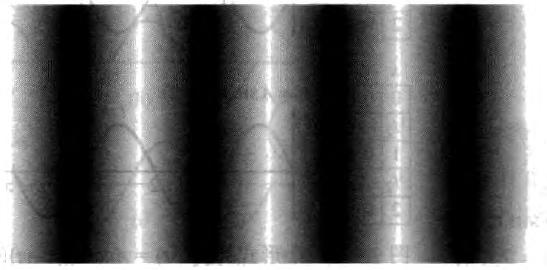
\includegraphics[height=120pt]{assets/image (41).jpg}
    \caption{\textbf{空间频率较低的正弦亮度分布}}\label{空间频率较低的正弦亮度分布}
    \end{figure}
    \end{minipage}
    \begin{minipage}{0.35\textwidth}
    \begin{figure}[H]\centering
    
\includegraphics[height=120pt]{assets/image (42).jpg}
    \caption{\textbf{空间频率较高的正弦亮度分布}}\label{空间频率较高的正弦亮度分布}
    \end{figure}
\end{minipage}
\end{definition}

\section{相位和相速度}
考虑任何一个一维波函数 $\psi(x,t) = A \sin(kx-vt + \varphi_0)$,$\varphi = kx+vt$ 称为相位,$\varphi_0$ 称为初相。

由热力学中的偏微分关系,我们定义相速度:
\begin{equation}
    \left(\frac{\partial x }{\partial t }\right)_{\varphi} = -\frac{\left(\frac{\partial \varphi }{\partial t }\right)_{x}}{\left(\frac{\partial \varphi }{\partial x }\right)_{t}}
\end{equation}



\chapter*{附录 B. 标题}\addcontentsline{toc}{chapter}{附录 B. 标题}   % B 章节
\thispagestyle{fancy} 
\setcounter{section}{0}   
\renewcommand\thesection{B.\arabic{section}}   
\renewcommand{\thefigure}{B.\arabic{figure}} 
\renewcommand{\thetable}{B.\arabic{table}}

\section{支撑材料列表} 

\begin{center}
  这里插入一张图片(类似思维导图那种)
\end{center}

\begin{multicols}{2}  

    \begin{table}[H]\centering
    \caption{\textbf{中英文对照表}}
    \begin{tabular}{cccccccc}\toprule
        English & 中文 \\
        \midrule
        voltage            & 电压 \\
        current            & 电流 \\
        power              & 功率 \\
        resistance         & 电阻 \\
        conductance        & 电导 \\
        inductance         & 电感 \\
        capacitance        & 电容 \\
        frequency          & 频率 \\
        circuit            & 电路 \\
        circuit element    & 电流元件 \\
        signal             & 信号 \\
        circuit analysis   & 电路分析 \\
        circuit synthesis  & 电路综合 \\
        circuit design     & 电路设计 \\
        circuit topology   & 电路拓扑 \\
        \bottomrule
    \end{tabular}
    \end{table}
    
    \begin{table}[H]\centering
        \caption{\textbf{中英文对照表}}
        \begin{tabular}{cccccccc}\toprule
            English & 中文 \\
            \midrule
            voltage            & 电压 \\
            current            & 电流 \\
            power              & 功率 \\
            resistance         & 电阻 \\
            conductance        & 电导 \\
            inductance         & 电感 \\
            capacitance        & 电容 \\
            frequency          & 频率 \\
            circuit            & 电路 \\
            circuit element    & 电流元件 \\
            signal             & 信号 \\
            circuit analysis   & 电路分析 \\
            circuit synthesis  & 电路综合 \\
            circuit design     & 电路设计 \\
            circuit topology   & 电路拓扑 \\
            \bottomrule
        \end{tabular}
    \end{table}
\end{multicols} 
    

\section{这里是我的第二节附录}
% 注意:listing环境中手动输入的代码需要顶格写

\begin{matlablisting}
% MATLAB code here
x = 0:0.1:2*pi;
y = sin(x);
plot(x, y);
xlabel('x');
ylabel('sin(x)');
title('Sine Function');
% ... (MATLAB code here,最好是插入文件)
% MATLAB code here
x = 0:0.1:2*pi;
y = sin(x);
plot(x, y);
xlabel('x');
ylabel('sin(x)');
title('Sine Function');
% ... (MATLAB code here,最好是插入文件)
% MATLAB code here
x = 0:0.1:2*pi;
y = sin(x);
plot(x, y);
xlabel('x');
ylabel('sin(x)');
title('Sine Function');
% ... (MATLAB code here,最好是插入文件)
% MATLAB code here
x = 0:0.1:2*pi;
y = sin(x);
plot(x, y);
xlabel('x');
ylabel('sin(x)');
title('Sine Function');
% ... (MATLAB code here,最好是插入文件)
% MATLAB code here
x = 0:0.1:2*pi;
y = sin(x);
plot(x, y);
xlabel('x');
ylabel('sin(x)');
title('Sine Function');
% ... (MATLAB code here,最好是插入文件)
% MATLAB code here
x = 0:0.1:2*pi;
y = sin(x);
plot(x, y);
xlabel('x');
ylabel('sin(x)');
title('Sine Function');
% ... (MATLAB code here,最好是插入文件)% ... (MATLAB code here,最好是插入文件)% ... (MATLAB code here,最好是插入文件)% ... (MATLAB code here,最好是插入文件)% ... (MATLAB code here,最好是插入文件)A
% MATLAB code here
x = 0:0.1:2*pi;
y = sin(x);
plot(x, y);
xlabel('x');
ylabel('sin(x)');
title('Sine Function');
% ... (MATLAB code here,最好是插入文件)
\end{matlablisting}

\section{这里是我的第三节附录}
你好你好你好你好你好你好

\end{document}



% VScode 常用快捷键:

% F2:                       变量重命名
% Ctrl + Enter:             行中换行
% Alt + up/down:            上下移行
% 鼠标中键 + 移动:           快速多光标
% Shift + Alt + up/down:    上下复制
% Ctrl + left/right:        左右跳单词
% Ctrl + Backspace/Delete:  左右删单词    
% Shift + Delete:           删除此行
% Ctrl + J:                 打开 VScode 下栏(输出栏)
% Ctrl + B:                 打开 VScode 左栏(目录栏)
% Ctrl + `:                 打开 VScode 终端栏
% Ctrl + 0:                 定位文件
% Ctrl + Tab:               切换已打开的文件(切标签)
% Ctrl + Shift + P:         打开全局命令(设置)

% Latex 常用快捷键

% Ctrl + Alt + J:           由代码定位到PDF
% 


% Git提交规范:
% update: Linear Algebra 2 notes
% add: Linear Algebra 2 notes
% import: Linear Algebra 2 notes
% delete: Linear Algebra 2 notes














































































































































































































































































































































































































































































































































































































\end{document}

% VScode 常用快捷键:

% F2:                       变量重命名
% Ctrl + Enter:             行中换行
% Alt + up/down:            上下移行
% 鼠标中键 + 移动:           快速多光标
% Shift + Alt + up/down:    上下复制
% Ctrl + left/right:        左右跳单词
% Ctrl + Backspace/Delete:  左右删单词    
% Shift + Delete:           删除此行
% Ctrl + J:                 打开 VScode 下栏(输出栏)
% Ctrl + B:                 打开 VScode 左栏(目录栏)
% Ctrl + `:                 打开 VScode 终端栏
% Ctrl + 0:                 定位文件
% Ctrl + Tab:               切换已打开的文件(切标签)
% Ctrl + Shift + P:         打开全局命令(设置)

% Latex 常用快捷键

% Ctrl + Alt + J:           由代码定位到PDF
% 


% Git提交规范:
% update: Linear Algebra 2 notes
% add: Linear Algebra 2 notes
% import: Linear Algebra 2 notes
% delete: Linear Algebra 2 notes
